% Figure from MATH 556 notes, section 9. Compile with the notes preamble.
\begin{tikzpicture}[scale=5, >=stealth]
    \draw[thick] (0,0) -- (1,0);
    \foreach \n in {2,...,14} \fill ({1/\n},0) circle (0.35pt);
    \draw[fill=white] (0,0) circle (0.7pt);
    \draw[fill=white] (1,0) circle (0.7pt);
    \node[below] at (0,-0.02) {$0 \notin M$};
    \node[below] at (1,-0.02) {$1 \notin M$};
    \node[above] at (0.5,0.02) {$\tfrac12$};
    \node[above] at (0.3333,0.02) {$\tfrac13$};
    \node[above] at (0.25,0.02) {$\tfrac14$};
    \draw[->, red!75!black] (0.35,-0.07) -- (0.12,-0.07);
    \node[red!75!black, anchor=west] at (0.36,-0.07) {$x_n = \tfrac1n \to 0$};
\end{tikzpicture}
